%\chapter{The Basics of Loading and Manipulating Data}
\chapter{The Invocation and Metamorphosis of Data}

\lettrine{H}{eed} this warning: The data frame is your most loyal servant \ldots{} and your most treacherous foe. It will be the focus of this chapter. Treat it with reverence, for a single misstep may awaken errors best left entombed.

Chapter 1 stated that data frames are essential for keeping a host of related information stored in a well organized manner that is easy to manipulate. When printed to the console, data frames present as a familiar spreadsheet-like structure that can be created, subset, and altered in various ways (see section \ref{sec:data_frames} for details). Moreover, in chapter 1, we saw how a data frame can be constructed by manually entering values with R code. And, for all but the smallest of data sets, this method is time-consuming and highly prone to error. A better strategy is to take an existing file of information and import that directly into R as a data frame or, depending on the nature of the data, as a list, matrix, array, or table. A data frame is usually going to be the optimal choice and will be the primary focus of this chapter.

Data can come in all kinds of different layouts and file formats and, in this respect, R has the ability to handle pretty much any scenario that might arise. This chapter will, for the most part, work under the assumption that the  kind of data that you need to work with is in a conventional ``spreadsheet-style'' of format. That is to say, like the \R{msleep} data used in Chapter 2, you have a bunch of rows and a bunch of columns, and each cell contains just a single value.

\section{Spreadsheet Software}
\label{sec:spreadsheet_soft}

When it comes to spreadsheets, there are many different file formats.  Pretty much every spreadsheet application has its own specific file type that is tailored to its unique purpose and platform. For instance, \textit{Microsoft's Excel} spreadsheet application has its own proprietary format called the \texttt{.xlsx} file format. The stock spreadsheet application on Macintosh computers, called \textit{Numbers}, use the \texttt{.NUMBERS} file format. And if you use an open-source spreadsheet software like \textit{Libre Office's Calc} application, you may be familiar with the \texttt{.ods} file format.

As everyone who is reading this doubtlessly appreciates, spreadsheet applications like Microsoft's Excel, Numbers, Libre Office's Calc, etc., do more than just structure your data in a big table (which is all a spreadsheet is).  They allow you to do things like perform calculations, adjust cell colours, add images, insert comments, etc. And all of this extra stuff is saved, in one form or another, inside the specific file associated with that software. These features make applications like Microsoft's Excel, for instance, a great tool for basic tasks like balancing the household budget.  However, for serious data analysis that requires the use of large data sets and complex or heavy calculations, this kind of software is going to be more of a hindrance than a help. Adding in all of those layers of additional functionality is going to increase your file sizes, inflate your load times, create restrictions on how much information can be contained within your spreadsheet, and will increase the chance of a glitch occurring. Additionally, and most importantly, both the analyses and the data are all contained within the same file, which makes it very easy to irrevocably damage your original data set, often without even realizing it. The fact is, we should care about analyzing our data efficiently and safely, not making it look pretty in what amounts to a fancy table, and this is one of the key benefits of using R.

From the point of view of R, a spreadsheet is just a way of displaying the raw information it is analysing, and nothing more. The analysis of that information is what R does. Technically then, we should not be referring to something as a ``spreadsheet file,'' but rather a ``data file.'' The spreadsheet aspect of all of this is more about how the data is structured for our viewing. However, data does not necessarily need to be viewed as a spreadsheet - it can be viewed in all kinds of different ways. It is just that a spreadsheet is usually the most convenient and intuitive way to view it and talk about it.

\section{Using an Ethical File Format}
\label{sec:ethical_file}

As noted above, there are a variety of different spreadsheet file types data could be formatted as (\texttt{.xlsx}, \texttt{.ods}, etc). To remain consistent with open-science principles \parencite{UNESCO_open_sci}, best practice dictates that you work with your data in a file format that is both universally recognized across applications and will also stand the test of time in terms of compatibility.  In other words, we want to (ideally) work with a file format that has no immediate risk of becoming obsolete and can be read by multiple computers on multiple platforms without forcing the user to pay for some proprietary application. Along these lines, the most widely used and recognized format is the \texttt{.csv} file format.

\section{The .CSV Format}

``CSV'' stands for ``comma separated values.'' It gets its name from the fact that it is, quite literally, nothing more than a generic text document that uses commas to denote a tabular (spreadsheet structure) in the data.\footnote{``Tabular'' and ``spreadsheet'' mean the same thing here.} This is easiest to see with an example. The GitHub repository for this book contains a file called \R{MM\_Madison\_wide.csv}. The file is located within the \R{data} directory at \R{./data/ch-3/MM-candy/}. The GitHub repo can be accessed at the following URL: 

\begin{center}
\url{https://github.com/statistical-grimoire/book/}
\end{center}

\noindent
It contains measurements of the colour distribution of M\&M Milk Chocolate candies, collected by Josh Madison for his blog \parencite{Madison2007}. Josh purchased a case of Milk Chocolate M\&M's (which is 48 separate packages of M\&M's) and counted how many of each M\&M colour (blue, brown, green, orange, red, yellow) were contained in each pack. He did this, ostensibly, to evaluate a theory he had about the manufacturing process of the candies.\footnote{Or, more realistically, he just wanted a excuse to purchase and eat Milk Chocolate M\&M's guilt free.}

Upon opening the file within GitHub,\footnote{\url{https://github.com/statistical-grimoire/book/blob/main/data/ch-3/MM-candy/MM_Madison_wide.csv}} you will see that it displays the file's contents in a fairly typical spreadsheet layout (see Table \ref{table:mm_madison} for an example displaying the first 6 rows).

\vspace{1em}

% latex table generated in R 4.4.1 by xtable 1.8-4 package
% Wed Jul 24 10:28:44 2024
\begin{table}[H]
\centering
\begin{tabular}{rrrrrrrrrr}
  \hline
 & pkg & weight\_oz & year & blue & brown & green & orange & red & yellow \\ 
  \hline
1 & 1.00 & 1.69 & 2007 &  13 &   7 &  12 &   9 &   7 &   8 \\ 
  2 & 2.00 & 1.69 & 2007 &   8 &   3 &  13 &  13 &  10 &   6 \\ 
  3 & 3.00 & 1.69 & 2007 &   8 &  10 &  11 &  10 &   5 &  10 \\ 
  4 & 4.00 & 1.69 & 2007 &  14 &   4 &   6 &  14 &   7 &   9 \\ 
  5 & 5.00 & 1.69 & 2007 &   6 &   8 &  10 &  12 &   8 &   8 \\ 
  6 & 6.00 & 1.69 & 2007 &   7 &  11 &  13 &   7 &   4 &  13 \\ 
   \hline
\end{tabular}
\caption{First 6 rows of the \R{MM\_Madison\_wide.csv} data displayed in a spreadsheet structure.}
\label{table:mm_madison}
\end{table}

\vspace{1em}

\noindent
However, this is just how GitHub presents \texttt{.csv} files. The actual raw data is a basic text document that separates individual values with a comma. We can see this more clearly if we click the button labelled ``Raw'' which will present the file in its unaltered (i.e., raw) text format. The first 6 rows can be seen below

\vspace{1em}
\begin{listing}[H]
\begin{raw}
pkg,weight_oz,year,blue,brown,green,orange,red,yellow
1,1.69,2007,13,7,12,9,7,8
2,1.69,2007,8,3,13,13,10,6
3,1.69,2007,8,10,11,10,5,10
4,1.69,2007,14,4,6,14,7,9
5,1.69,2007,6,8,10,12,8,8
6,1.69,2007,7,11,13,7,4,13
...
\end{raw}
\caption*{Example of the \R{MM\_Madison\_wide.csv} data file displayed in its raw text format. Only the first six rows are shown.}
\end{listing}

\vspace{1em}

Comparing the two versions it can readily be seen how the commas are functioning. They separate individual cells/columns and each new line represents a new row in the spreadsheet. This not only makes it easy to read \texttt{.csv} files within a basic text editor, but create them as well. Just save (or rename) the text document with a \texttt{.csv} file extension (which you may need to configure your computer to display). Alternatively, if you have a good spreadsheet software on your computer, they will always have the ability to \textit{``Save As''} a \texttt{.csv} file or \textit{``Export''} to one. For instance, the save menu of Microsoft Excel will present the user with a drop down list of potential file types it can save as and (as of writing this) has four different versions of \texttt{.csv} files (the best option is the one labelled ``UTF-8 (Comma delimited)''). By contrast the Numbers application on a Mac will not permit a spreadsheet to save as anything other than a \texttt{.NUMBERS} file, but will allow you to export your saved spreadsheet as a \texttt{.csv}. Just select \textit{File $\rightarrow$ Export To $\rightarrow$ CSV... }

\section{Delimiters}

In the case of the \R{MM\_Madison\_wide.csv} file, the comma is functioning as a \gls{delimiter}; which is to say it is a character that defines the limits of (i.e., it ``delimits'') individual values. Commas are not the only characters that can be used to delimit, any character can technically be used. Other common delimiters include semicolons (;) and tab-key spaces. Semicolons are often used when the data is logged with commas representing decimal points instead of periods (e.g., 13.666 = 13,666), which is a frequent practice in many countries. Oddly, when a delimited file uses semicolons, it is still often given a \texttt{.csv} file extension despite it being a completely different character.  In R, to avoid confusion, the convention is to refer to these semicolon delimited files as \R{csv2} files in function names (e.g., \R{write\_csv()} would use a comma to delimit whereas \R{write\_csv2()} would use a semicolon).

Tab spaces (i.e., pressing ``tab'' on your keyboard), are also frequently employed as a delimiter, but these are usually denoted as .TSV files (i.e., tab separated values). In fact, the name for the keyboard key ``tab'' comes from the the verb ``tabulate'' because the key facilitated easier generation of tables when working on a typewriter. Prior to the tab key's development, the space bar had to be repeatedly pressed to advance the typewriter's carriage to align columns appropriately. 

If you were to save the \R{MM\_Madison\_wide} data set as a \texttt{.tsv} file and open it within a generic text editor, you would see something very similar to the following ...

\vspace{1em}
\begin{listing}[H]
\begin{raw}
pkg	weight_oz	year	blue	brown	green	orange	red	yellow
1	1.69	2007	13	7	12	9	7	8
2	1.69	2007	8	3	13	13	10	6
3	1.69	2007	8	10	11	10	5	10
4	1.69	2007	14	4	6	14	7	9
5	1.69	2007	6	8	10	12	8	8
6	1.69	2007	7	11	13	7	4	13
...
\end{raw}
\caption*{Example of the \R{MM\_Madison\_wide.csv} data file displayed in its raw text format if it were a .TSV file. Only the first six rows are shown.}
\end{listing}
\vspace{1em}

Notice that the tabular separation gives the file a much more grid-like aesthetic that is easier to read. Incorporating spaces into the text file can be used to further refine the alignment.

\section{Reading a CSV File into R}

Now that we have a good sense of what a \texttt{.csv} file is we should discuss how to load it into R as a data frame object so we can conduct our analyses. To begin with, you should download \R{MM\_Madison\_wide.csv} from the aforementioned GitHub repo by simply clicking the ``down arrow'' icon labelled ``Download raw file.'' Once downloaded, simply place the file inside your working directory.\footnote{If you are unsure what a ``working directory'' is see section \ref{sec:dir}} Depending on the browser you are using you may have to hunt around for the download option. For instance, if you are using Safari, you may have to select ``more file actions.''

With the file in its appropriate location you can simply run the function \R{read\_csv()} and give it the full name (with extension) of your file. This will create a data frame object in R. However, \R{read\_csv()} is a function that belongs to the \textit{readr} package which is part of the \textit{tidyverse}, so if you do not have the \textit{tidyverse} loaded, this will not work. In order to easily call our loaded data, we will assign it the name \R{mm\_df}.

\begin{inR}
library(tidyverse)
mm_df <- read_csv("MM_Madison_wide.csv")
\end{inR}

\begin{outR}
Rows: 48 Columns: 9                                                                                                      
Column specification 

Delimiter: ","
dbl (9): pkg, weight_oz, year, blue, brown, green, orange, red, yellow

Use `spec()` to retrieve the full column specification for this data.
Specify the column types or set `show_col_types = FALSE` to quiet this message.
\end{outR}

Running the above code presents us with some useful information about the data set we have loaded.  We can see that it has 48 rows and 9 columns, uses a \R{,} as a delimiter, and the 9 columns all consist of \R{dbl} values, which is a shorthand way of referring to \textit{double-precision number}. To simplify a complex story, R has multiple types of \textit{numeric} objects; i.e., it has multiple ways of representing a number. A \textit{double}, as its often referred to, is one such representation. If that is confusing, do not worry, what is important to take away from the output is that \R{dbl} means the 9 columns all contain numeric values.

Running \R{mm\_df} will print the data frame to the console.

\begin{inR}
mm_df
\end{inR}

\begin{outR}
# A tibble: 48 × 9
     pkg weight_oz  year  blue brown green orange   red yellow
   <dbl>     <dbl> <dbl> <dbl> <dbl> <dbl>  <dbl> <dbl>  <dbl>
 1     1      1.69  2007    13     7    12      9     7      8
 2     2      1.69  2007     8     3    13     13    10      6
 3     3      1.69  2007     8    10    11     10     5     10
 4     4      1.69  2007    14     4     6     14     7      9
 5     5      1.69  2007     6     8    10     12     8      8
 6     6      1.69  2007     7    11    13      7     4     13
 7     7      1.69  2007     8     7    13      8     7      9
 8     8      1.69  2007    12    10     6      8     8      9
 9     9      1.69  2007     6     9    12     14     8      6
10    10      1.69  2007     7     8    12     10    11      7
# 38 more rows
# Use `print(n = ...)` to see more rows
\end{outR}

You can now subset and manipulate \R{mm\_df} like we did in Chapter 1 when we first discussed data frames (see section \ref{sec:data_frames}). For instance, if we wanted to look at the mean number of green M\&M's across all the packages we could simply run:

\begin{inR}
mean(mm_df$green)
\end{inR}
\begin{outR}
[1] 10.0625
\end{outR}

\subsubsection{\texttt{read.csv()} vs. \texttt{read\_csv()}}

To load the M\&M data frame above, we used the function \R{read\_csv()}, which is part of the \textit{tidyverse}. However, base R as similar function, \R{read.csv()}, that will do essentially the same thing - it will read a \texttt{.csv} file in to R. For most use cases there is little advantage to adopting one function over the other, but if you have the \textit{tidyverse} loaded, you may as well use \R{read\_csv()} because it does have some big advantages. First, it offers excellent customization options, which are particularly useful when loading very large datasets or merging multiple datasets. Second, it alerts you to any issues encountered during the loading process. Third, it performs much faster under heavy loads than its base R counterpart, even providing a progress bar when reasonable to do so. Finally, it stores the data as a \textit{tibble} which will be discussed later.

\subsection{Reading Other File Types into R}

If your data is delimited by some character other than a comma (e.g., a semicolon, tab, backslash, etc.), there is a more general function that can be employed called \R{read\_delim()} which allows you to specify any delimiter (i.e., separator) using the argument \R{delim}. For instance, we could have loaded the M\&M data in the following way:

\begin{inR}
mm_df <- read_delim("MM_Madison_wide.csv", delim = ",")
\end{inR}

\vspace{1em}

\noindent
If your text document was separated by semicolons you would just include \R{delim = ";"}, if it was separated using tabs you would just \R{delim = "\textbackslash t"}, and so on. 

One thing that is worth appreciating about delimited files is that their file extension (e.g., the \texttt{.csv} or \texttt{.tsv} at the end of the file name) is irrelevant to how R reads the file. As has been previously emphasized, \texttt{.csv} files and \texttt{.tsv} files for instance, are just generic text documents, nothing more. This means you may see them with the file extension \texttt{.txt}, but that will not impact how any of the above functions operate.

Now, what would you do if you wanted to load a Microsoft Excel spreadsheet file (i.e., a \texttt{.xlsx} file) into R directly? Well as per the discussion on spreadsheets and ethical file formats (see section \ref{sec:spreadsheet_soft} and \ref{sec:ethical_file}), the best practice is to save it as a \texttt{.csv} using Excel and load that new file directly into R. However, should you wish to eschew this advice, the \textit{tidyverse} does have a package called \textit{readxl} with functions that will allow you to do this. This is not part of the nine core packages, so it will need to be loaded using the \R{library()} function. A word of warning is in order though. As well made as the \textit{readxl} package is, reading \texttt{.xlsx} files directly will, almost certainly, cause more problems than it solves. These files are not intended to be read by anything other than Excel and Microsoft does not want them read by anything other than Excel. Thus, by loading the \texttt{.xlsx} file directly into R, you are (computationally speaking) picking an unnecessary fight with Microsoft. Nine times out of ten, you will win that fight thanks to \textit{readxl}, but you will still probably end up with some nasty bruises and scars.

\section{Tibbles vs. Data Frames}

In the output for \R{mm\_df} (and the \R{msleep} data from chapter 2) you can see that the output printed to the console specifies that we are looking at something called a \gls{tibble}: \R{\# A tibble: 48 x 9}. The output also helpfully displays the dataset's dimensions and the class of object contained within each column. This is in contrast to the data frame created in chapter 1, which did not do any of that for us. In the \textit{tidyverse's} own words, a tibble is a ...

\begin{displayquote}
\headingfont
%\large
modern reimagining of the data.frame, keeping what time has proven to be effective, and throwing out what is not. Tibbles are data.frames that are lazy and surly: they do less (i.e. they don’t change variable names or types, and don’t do partial matching) and complain more (e.g. when a variable does not exist). This forces you to confront problems earlier, typically leading to cleaner, more expressive code. Tibbles also have an enhanced print( ) method which makes them easier to use with large datasets containing complex objects.

- \textit{\url{https://tibble.tidyverse.org/}}

\vspace{-1em}
(2024/07/28)

\end{displayquote}

In terms of basic usage, tibbles function almost identically to the classic data frame discussed in chapter 1. For instance, we can re-create chapter 1's data frame as a tibble using an identical syntax.

\begin{inR}
df <- tibble(
  Subject = 1:10,
  Group = c("Exp", "Cont", "Exp", "Cont", "Exp", "Exp",
            "Cont", "Exp", "Cont", "Cont"),
  Value = c(-0.36,  0.28,  1.54,  0.51, -1.28,  1.15,
            -2.22, -0.51,  NA, -1.04)
)

df
\end{inR}

\begin{outR}
# A tibble: 10 × 3
   Subject Group Value
     <int> <chr> <dbl>
 1       1 Exp   -0.36
 2       2 Cont   0.28
 3       3 Exp    1.54
 4       4 Cont   0.51
 5       5 Exp   -1.28
 6       6 Exp    1.15
 7       7 Cont  -2.22
 8       8 Exp   -0.51
 9       9 Cont  NA   
10      10 Cont  -1.04
\end{outR}

\noindent
There are a number of interesting differences between tibbles and data frames, but nothing that merits any in depth discussion for a beginner with R. What is perhaps worth noting is that it is easy to switch between the two should the need arise. For example, to convert our tibble \R{df} to a data frame, we can simply use the \R{as.data.frame()} function in R.

\begin{inR}
# tibble to data frame
df <- as.data.frame(df)
df
\end{inR}
\begin{outR}
   Subject Group Value
1        1   Exp -0.36
2        2  Cont  0.28
3        3   Exp  1.54
4        4  Cont  0.51
5        5   Exp -1.28
6        6   Exp  1.15
7        7  Cont -2.22
8        8   Exp -0.51
9        9  Cont    NA
10      10  Cont -1.04
\end{outR}

\noindent
To convert it back to a tibble ...
\begin{inR}
# data frame to tibble
df <- as_tibble(df)
df
\end{inR}
\begin{outR}
# A tibble: 10 × 3
   Subject Group Value
     <int> <chr> <dbl>
 1       1 Exp   -0.36
 2       2 Cont   0.28
 3       3 Exp    1.54
 4       4 Cont   0.51
 5       5 Exp   -1.28
 6       6 Exp    1.15
 7       7 Cont  -2.22
 8       8 Exp   -0.51
 9       9 Cont  NA   
10      10 Cont  -1.04
\end{outR}

\subsection{Displaying Tibbles in the Console}

\subsubsection{Tibble Dimensions}

Given the limited screen space and the large size of most datasets, tibbles are designed to display only the first 10 rows when printed to the console, making it easier for users to work with their data.

Generally, if you want to view an entire data set, the best practice is not to display it in the console but rather use R's \R{View()} function which opens it in a spreadsheet style viewer. That being said, many people will still find the number of rows displayed by a tibble within the console lacking, particularly if you are working on anything other than a small laptop. For this reason, the 10 row limit is a behaviour which can be circumvented in various ways. One simple way is to make use of the \R{print()} function. For instance, if we want to display the first 20 rows we can simply run ...

\begin{inR}
print(mm_df, n = 20)
\end{inR}

\vspace{1em}

An alternative method is to change R's default display behaviour by setting the number using the \R{options()} function. You can set both a minimum and maximum number of rows to display.

\begin{inR}
options(
  pillar.print_min = 30,
  pillar.print_max = 30
)

mm_df
\end{inR}

\vspace{1em}

\noindent
If that method is your preference, then it is usually advisable to place the \R{options()} code at the top of your R script because it only needs to be run once.\footnote{If you are wondering why we specify \R{pillar...} to set rows, it's because \textit{pillar} is a package in the tidyverse.}

What if you wanted to display every single row each time you print a tibble? Well, recall that R represents infinity in the positive direction as (\R{Inf}). We can use that to our advantage here:

\begin{inR}
options(pillar.print_min = Inf)

mm_df
\end{inR}

\vspace{1em}

What about columns though? Well, interestingly tibbles will actually conform to the size of your console screen.  So if you can only fit five columns on screen, the tibble will only display those five and notify you of the others not displayed beneath the output. This is done to preserve the ``rectangleness'' of the data so it can be visualized appropriately. This also stands in stark contrast to how base R's data frames behave, which will stack columns on top of each other with no consideration of column or row space. Admittedly, its nice to have all that information displayed, but it comes at the cost of being difficult for a human to visually parse. That being said, if you wanted your tibbles to behave like this and always display all columns, you can just add an additional argument, \R{pillar.width = Inf}, to the \R{options()} function:

\begin{inR}
options(
  pillar.print_min = 30,
  pillar.print_max = 30,
  pillar.width = Inf
)

mm_df
\end{inR}

\vspace{1em}

\noindent
However, if you wanted a more temporary solution, you can just add a \R{width} argument to the \R{print()} function. E.g., 

\begin{inR}
print(mm_df, n = 30, width = Inf)
\end{inR}

\vspace{1em}

\subsubsection{Understanding Significant Digits}
\label{sec:sig_digs}

To save space and facilitate easier reading, both tibbles and data frames will round values with many decimal values. Though, in the case of tibbles, they do not just simply round to a preset number of digits.  To illustrate what tibbles are doing in this respect, recall that R has a built-in constant for $\pi$.

\begin{inR}
pi
\end{inR}
\begin{outR}
[1] 3.141593
\end{outR}

\noindent
Using that, we will create a simple data frame that repeats $\pi$ four times within a single column.

\begin{inR}
pi_df <- tibble(pie = rep(pi, 4))
pi_df
\end{inR}
\begin{outR}
# A tibble: 10 × 1
     pie
   <dbl>
 1  3.14
 2  3.14
 3  3.14
 4  3.14
\end{outR}

\noindent
One thing that will be noticed is that the tibble is only displaying $\pi$ to two decimal places. However, all of the digits still exist in R's memory and any calculations you do will take those unseen digits into account. For instance, if we isolate the first row's value you can see that all the digits of $\pi$ are displayed.

\begin{inR}
pi_df$pie[1]
\end{inR}
\begin{outR}
[1] 3.141593
\end{outR}

\noindent
It is important to understand that tibbles do not strictly control the handling of decimals. Instead, they work with \textit{significant digits}.  This allows the tibble to preserve its desired ``rectangleness,'' giving it cleaner looking columns. Since tibbles default to three significant digits, $\pi$ will only display as 3.14. 

As a refresher of primary school math, with significant digits, everything in front of the decimal point is always displayed, but each number in front of that decimal point uses up a significant digit (a.k.a. a ``sig dig''). For instance, if you had a number like 666.13.  Displaying that to two sig digs would give you 666.  Displayed to three sig digs would again be 666. Displayed to four sig digs would be 666.1. Five sig digs would be 666.13. Six sig digs would be 666.130. Seven would be 666.1300, and so on.

To increase the number of sig digs shown within a tibble we can simply add another argument to the \R{options()} function:

\begin{inR}
options(pillar.sigfig = 16)
pi_df
\end{inR}
\begin{outR}
# A tibble: 10 × 1
                   pie
                 <dbl>
 1 3.141592653589793e0
 2 3.141592653589793e0
 3 3.141592653589793e0
 4 3.141592653589793e0
\end{outR}

Because of limitations of 64-bit computing, a tibble is not going let you exceed 16 sig digs and in certain cases will display results in scientific notation. In this case we see some scientific notation, but it is to the power of 0, so it can be ignored.

\section{Wide Data vs. Tidy Data}

\subsection{Wide Data}
\label{sec:wide_data}

Looking at the \R{MM\_Madison\_wide.csv} loaded at the outset of this chapter, you can see that the data is laid out in a fairly logical manner. Each row corresponds to a different package of M\&Ms and we can clearly see how many M\&Ms of a particular colour are in each package by examining the columns named, blue, brown, green, etc.

\begin{inR}
mm_df
\end{inR}

\begin{outR}
# A tibble: 48 × 9
     pkg weight_oz  year  blue brown green orange   red yellow
   <dbl>     <dbl> <dbl> <dbl> <dbl> <dbl>  <dbl> <dbl>  <dbl>
 1     1      1.69  2007    13     7    12      9     7      8
 2     2      1.69  2007     8     3    13     13    10      6
 3     3      1.69  2007     8    10    11     10     5     10
 4     4      1.69  2007    14     4     6     14     7      9
 5     5      1.69  2007     6     8    10     12     8      8
 6     6      1.69  2007     7    11    13      7     4     13
 7     7      1.69  2007     8     7    13      8     7      9
 8     8      1.69  2007    12    10     6      8     8      9
 9     9      1.69  2007     6     9    12     14     8      6
10    10      1.69  2007     7     8    12     10    11      7
# 38 more rows
# Use `print(n = ...)` to see more rows
\end{outR}

This style of layout makes it easy to do certain things with the data. For instance, if we wanted to know the mean number of red M\&Ms we could just run 

\begin{inR}
mean(mm_df$red)
\end{inR}

\begin{outR}
[1] 7.75
\end{outR}

If we wanted to obtain the mean of every column, we could use the \R{apply()} function. This function literally \textit{applies} a function of your choosing to either the columns or rows. So we could, for instance, apply the \R{mean()} function to each \textit{column}.

\begin{inR}
apply(mm_df, MARGIN = 2, FUN = mean)
\end{inR}

\begin{outR}
        pkg   weight_oz        year        blue       brown       green 
  24.500000    1.690000 2007.000000   10.020833    7.729167   10.062500 
     orange         red      yellow 
  11.333333    7.750000    7.687500 
\end{outR}

\noindent
The argument \R{FUN} specifies what function is applied. The argument \R{MARGIN} specifies whether that function is applied to the rows (\R{1}) or columns (\R{2}). In this case we are applying it to columns, so we specified \R{2}.

If you wanted to count how many M\&Ms are in each individual package, you could \textit{apply} the \R{sum()} function to the \textit{rows} - though, keep in mind that we would want to ignore \R{pkg}, \R{weight\_oz}, and \R{year} values when doing this. Luckily we can use what we learned about indexing in chapter 1 to ignore these columns (see section \ref{sec:df_Index}).

\begin{inR}
apply(mm_df[, 4:9], MARGIN = 1, FUN = sum)
\end{inR}

\begin{outR}
 [1] 56 53 54 54 52 55 52 53 55 55 54 54 52 55 55 53 55 56 54 57 55 54 55 57
[25] 53 54 54 57 56 57 55 54 54 57 56 56 55 55 55 53 55 54 54 53 54 54 55 55
\end{outR}

At a superficial glance, you can see that R makes it fairly easy to work with data in this kind of layout. However, we have not attempted anything fairly complicated here. The reality is that this layout, which we will refer to in this book as \gls{wide data}, is \textit{not} optimal for most types of analyses and plotting. Additionally, until you are actually in a position to do those kinds of analyses, it will be difficult to convince you of the truth of this - so you will just have to take that point on faith. Wide data spreads variables across multiple columns. In this case, you can treat of the colour of the M\&Ms here (blue, brown, green etc.) as a variable in its own right. We might call this variable simply ``type.'' That is to say, there is a ``blue'' \textit{type} of  M\&M, a ``brown'' \textit{type} of  M\&M, and so on.\footnote{A better variable name would be ``colour,'' but colour is also a plotting aesthetic and, later in the chapter, we will be plotting these data.  So to keep the plot's code a bit more intelligible, I'm refraining from using ``colour'' as the variable name.} There is also a second variable, which we could refer to as the ``amount'' of M\&M's, within each of the six colour type columns.

When organizing or arranging data, best practices dictate that you \textbf{restrict a single variable to a single column}. In this case, the variable ``type'' is being spread across six column headers. And the variable ``amount'' is spread within those six columns. To fix this, we can use the \textit{tidyverse} function \R{pivot\_longer()}.

\begin{inR}
mm_tidy <- pivot_longer(mm_df,
  cols = blue:yellow,
  names_to = "type", values_to = "amount"
)

mm_tidy
\end{inR}
\begin{outR}
# A tibble: 288 × 5
     pkg weight_oz  year type   amount
   <dbl>     <dbl> <dbl> <chr>   <dbl>
 1     1      1.69  2007 blue       13
 2     1      1.69  2007 brown       7
 3     1      1.69  2007 green      12
 4     1      1.69  2007 orange      9
 5     1      1.69  2007 red         7
 6     1      1.69  2007 yellow      8
 7     2      1.69  2007 blue        8
 8     2      1.69  2007 brown       3
 9     2      1.69  2007 green      13
10     2      1.69  2007 orange     13
11     2      1.69  2007 red        10
12     2      1.69  2007 yellow      6
# 276 more rows
\end{outR}

Notice a few differences with this pivoted data. There are now considerably more rows in the data, 288 vs. 48, and there are two new columns, \R{\$type} and \R{\$amount} which have replaced the six different colour type columns. In terms of the \R{pivot\_longer()} function we used, the most important argument we specified is the argument \R{cols}, as this defines which columns are going to be collapsed into a single column. Using the \R{:}, we specified a range of columns (i.e., from blue to yellow), but we could have also given it a vector of column names like so: \R{cols = c(blue, brown, green, orange, red, yellow)}.\footnote{The \textit{tidyverse} has numerous methods for selecting multiple columns that don't exist in base R.  For a rundown of each see the R documentation: \R{?tidyr\_tidy\_select}}

The arguments \R{names\_to} and \R{values\_to} just specify the name of the new columns and are not strictly required, but are good practice to include.


\subsection{Tidy data}

By collapsing the six colour columns into one, the data has ascended into a sacred arrangement known as \gls{tidy data} (or, as some heretics call it, ``the long format'').  Tidy data is a cornerstone of the \textit{tidyverse's} thaumaturgy and all tidy data adheres to three basic precepts:

\begin{minipage}{\textwidth}

\begin{enumerate}[label=\Roman*.]
\fontfamily{artemisia}\selectfont
    %\setlength\itemsep{-1em}
    %\large
    \item Each variable is a column; each column is a variable.
    \item Each observation is a row; each row is an observation.
    \item Each value is a cell; each cell is a single value.
\end{enumerate}
\end{minipage}

\noindent
It can be seen that the M\&M data now satisfies these three standards, as did the \R{msleep} data used in chapter 2. As we progress through the remainder of this chapter, it will become apparent that having your data in this tidy form will greatly facilitate both plotting and analysis. 


\section{Laying Pipe (The \texttt{|>} and \texttt{\%>\%} Operators)}

One of the most significant contributions of the \textit{tidyverse} to R has been its seamless implementation of what is known as `piping' syntax, which allows for an almost otherworldly level of efficiency. However, this is not to say that piping was a concept invented entirely by the \textit{tidyverse}. Rather, the \textit{tidyverse}'s consistent and innovative use of it brought its potential to light, leading to widespread adoption within the R community. The best evidence of this influence is the integration of piping into base R as of \href{https://stat.ethz.ch/pipermail/r-announce/2021/000670.html}{version 4.1.0}, released in 2021.\footnote{Although I have no direct evidence that the \textit{tidyverse} directly motivated the addition of the pipe operator to base R, it seems unlikely to be a coincidence given the ubiquity of \R{\%>\%} and the popularity of the \textit{dplyr} package.} But what exactly is 'piping'?

The essence of piping is that you are transferring the output of one thing to another. For instance, suppose we wanted to know the mean amount of different M\&M colours. We could of course insert the \R{\$amount} column into the mean function like so ...

\begin{inR}
mean(mm_tidy$amount)
\end{inR}
\begin{outR}
[1] 9.097222
\end{outR}

Alternatively, we could ``pipe'' (i.e., transfer) the \R{\$amount} column in our tidy data to the \R{mean()} function using R's pipe operator \R{|>}

\begin{inR}
mm_tidy$amount |> mean()
\end{inR}
\begin{outR}
[1] 9.097222
\end{outR}

\noindent We could then send that output to something like the \R{round()} function.

\begin{inR}
mm_tidy$amount |> 
    mean() |> 
    round(3)
\end{inR}
\begin{outR}
[1] 9.097
\end{outR}

As another example, suppose we wanted a tidy data frame that only contained the red M\&M type. The standard methodology would be to specify the data frame within the \R{filter()} function, like so ...

\begin{inR}
filter(mm_tidy, type == "red")
\end{inR}
\begin{outR}
# A tibble: 48 × 5
     pkg weight_oz  year type  amount
   <dbl>     <dbl> <dbl> <chr>  <dbl>
 1     1      1.69  2007 red        7
 2     2      1.69  2007 red       10
 3     3      1.69  2007 red        5
 4     4      1.69  2007 red        7
 5     5      1.69  2007 red        8
 6     6      1.69  2007 red        4
 7     7      1.69  2007 red        7
 8     8      1.69  2007 red        8
 9     9      1.69  2007 red        8
10    10      1.69  2007 red       11
# 38 more rows
\end{outR}

\noindent
Alternatively, we could pipe the data into the \R{filter()} function.

\begin{inR}
mm_tidy |> filter(type == "red")
\end{inR}
\begin{outR}
# A tibble: 48 × 5
     pkg weight_oz  year type  amount
   <dbl>     <dbl> <dbl> <chr>  <dbl>
 1     1      1.69  2007 red        7
 2     2      1.69  2007 red       10
 3     3      1.69  2007 red        5
 4     4      1.69  2007 red        7
 5     5      1.69  2007 red        8
 6     6      1.69  2007 red        4
 7     7      1.69  2007 red        7
 8     8      1.69  2007 red        8
 9     9      1.69  2007 red        8
10    10      1.69  2007 red       11
# 38 more rows
\end{outR}

In addition to this, suppose you did not want the \R{\$weight\_oz} or \R{\$year} column in the output. To achieve this, this output could be further piped into the \textit{tidyverse's} \R{select()} function which allows you to grab specific columns.

\begin{inR}
mm_tidy |> 
  filter(type == "red") |>
  select(pkg, type, amount)
\end{inR}
\begin{outR}
# A tibble: 48 × 3
     pkg type  amount
   <dbl> <chr>  <dbl>
 1     1 red        7
 2     2 red       10
 3     3 red        5
 4     4 red        7
 5     5 red        8
 6     6 red        4
 7     7 red        7
 8     8 red        8
 9     9 red        8
10    10 red       11
# 38 more rows
\end{outR}

Now that the logic of piping is clear, it is worth reiterating that the \R{|>} operator is a relatively new arrival in base R. Prior to this, the convention would be to use the \textit{tidyverse's} pipe operator \R{\%>\%} instead. This comes from a package called \textit{magrittr}, which contains a variety of pipes for different purposes, but the most significant of these is \R{\%>\%}. Before R version  4.1.0, \R{\%>\%} was the de facto pipe used by the R community at large. However, the recommended wisdom now (even by the keepers of the \textit{tidyverse}) is to use base R's pipe and not \textit{magrittr's}. That being said, many are unaware of this update to base R and much of the help documentation on websites like \href{https://stackoverflow.com/}{stack overflow} still use \textit{magrittr's} \R{\%>\%}. In terms of functionality, there is little meaningful difference between \R{|>} and \R{\%>\%} and all of the above code could have been written using \R{\%>\%}.

The above examples nicely show how the pipe operator works, but we should consider a more realistic use case to illustrate its versatility. 

\subsection{Data Manipulation Example}

\subsubsection{Summarising the Data}

The M\&M data we loaded earlier was of course in the wide format originally, which is rarely needed. So what we could have done instead is loaded that data in to R using \R{read\_csv}, then pipe it to the \R{pivot\_longer()} function and, if we wanted to, pipe that to the \R{select()} function to avoid keeping irrelevant columns.

\begin{inR}
mm_data <- read_csv("MM_Madison_wide.csv") |>
  pivot_longer(cols = blue:yellow, names_to = "type", values_to = "amount") |>
  select(pkg, type, amount)

mm_data
\end{inR}
\begin{outR}
# A tibble: 288 × 3
     pkg type   amount
   <dbl> <chr>   <dbl>
 1     1 blue       13
 2     1 brown       7
 3     1 green      12
 4     1 orange      9
 5     1 red         7
 6     1 yellow      8
 7     2 blue        8
 8     2 brown       3
 9     2 green      13
10     2 orange     13
# 278 more rows
\end{outR}

It is worth emphasizing the utility of the pipe operator here: It allowed us to get our data into the form we wanted without creating and calling multiple different objects in memory. Only one object was created, \R{mm\_data}. Moreover, the ``arrow-like'' notation of the pipe \R{|>} nicely shows the workflow, i.e., logic, of our code.

Now suppose we wanted to compute some summary statistics for this data set.  For instance, maybe we want to know the mean amount of each type of M\&M. This is where the \textit{tidyverse's} functions \R{group\_by()} and \R{summarise()} become extremely useful. Both of these functions, as well as the \R{filter()} and \R{select()} functions we have been using, come from the \textit{dplyr} package in the \textit{tidyverse}. 

\begin{figure}[h]
    \centering
\begin{mdframed}[style = miscFrame, frametitle = Box 3.1: Why is it called \textit{dplyr}?]

Generally, the names of R packages are relatively intuitive or are based on an initialism of some kind. The \textit{dplyr} package is an exception to that. The package's strange name is a reference to both pliers (the tool) and a family of functions based around the \R{apply()} function that we briefly used in section \ref{sec:wide_data}. The ``d'' refers to data frames. i.e., it is as if you are taking a pair of pliers to data frames.

\vspace{1em}

A common go-to strategy of programmers generally is to use for-loops to do much of the computational grunt work. For-loops just repeatedly execute a set of code until some condition has been satisfied. While for-loops can be used in R, its users often prefer to take a different, more efficient, ``vectorized'' approach. The goal is to use what are called \glspl{functional}. These are functions that accept another function as an input and produce a vector as output. That is precisely what the \R{apply()} function and its relatives like \R{lapply}, \R{sapply}, \R{vapply} do. R is incredibly adept at working with vectors, matrices, and arrays, and \textit{dplyr's} functions are all based around a strategy of using functionals for data manipulation.

\end{mdframed}
\end{figure}

We will begin with the \R{summarise()} function which is used to create a data frame based on columns/variables in your data.

\begin{inR}
mm_data |> 
  summarise(m = mean(amount))
\end{inR}

\begin{outR}
# A tibble: 1 × 1
      m
  <dbl>
1  9.10
\end{outR}

The code we have written is telling the \R{summarise()} function to apply the \R{mean()} function to the \R{\$amount} column. When it did this, it also created a new data frame and stored that calculation as a column called \R{\$m} (though, we could have named the column whatever we wanted).\footnote{If you are obtaining a giant value like \R{9.09722222222222e0} you probably forgot to reset the significant digits back to something reasonable. See section \ref{sec:sig_digs}.}

At present, none of this may not seem terribly useful; however, we can make it more useful by including the \R{group\_by()} function which will tell R to literally ``group by'' categories found in a different column or set of columns. Specifically, we can tell it to group by \R{\$type} and then summarise the data.

\begin{inR}
mm_data |> 
  group_by(type) |>
  summarise(m = mean(amount))
\end{inR}
\begin{outR}
# A tibble: 6 × 2
  type       m
  <chr>  <dbl>
1 blue   10.0 
2 brown   7.73
3 green  10.1 
4 orange 11.3 
5 red     7.75
6 yellow  7.69
\end{outR}

We can now see the mean of each type in the data set and if we wanted, we could create another column showing how many M\&M's of each type there are in total by taking the sum of all the blue M\&M's, the sum of all the brown M\&M's and so on.

\begin{inR}
mm_data |>
  group_by(type) |>
  summarise(
    m = mean(amount),
    tot_type = sum(amount)
  )
\end{inR}
\begin{outR}
# A tibble: 6 × 3
  type       m tot_type
  <chr>  <dbl>    <dbl>
1 blue   10.0       481
2 brown   7.73      371
3 green  10.1       483
4 orange 11.3       544
5 red     7.75      372
6 yellow  7.69      369
\end{outR}

If we wanted to add in a column that represented the total amount of M\&M's across all the packages (ignoring type) we could take the sum of the entire amount column ...

\begin{inR}
sum(mm_data$amount)
\end{inR}
\begin{outR}
[1] 2620
\end{outR}

\noindent
and include that in the \R{summarise()} function.

\begin{inR}
mm_data |>
  group_by(type) |>
  summarise(
    m = mean(amount),
    tot_type = sum(amount),
    tot_overall = sum(mm_data$amount)
  )
\end{inR}
\begin{outR}
# A tibble: 6 × 4
  type       m tot_type tot_overall
  <chr>  <dbl>    <dbl>       <dbl>
1 blue   10.0       481        2620
2 brown   7.73      371        2620
3 green  10.1       483        2620
4 orange 11.3       544        2620
5 red     7.75      372        2620
6 yellow  7.69      369        2620
\end{outR}

With the columns \R{\$tot\_type} and \R{\$tot\_overall} we could determine the percentage of each M\&M type by just doing the math inside the \R{summarise()} function.

\begin{inR}
mm_data |>
  group_by(type) |>
  summarise(
    m = mean(amount),
    tot_type = sum(amount),
    tot_overall = sum(mm_data$amount),
    percent = tot_type / tot_overall * 100
  )
\end{inR}
\begin{outR}
# A tibble: 6 × 5
  type       m tot_type tot_overall percent
  <chr>  <dbl>    <dbl>       <dbl>   <dbl>
1 blue   10.0       481        2620    18.4
2 brown   7.73      371        2620    14.2
3 green  10.1       483        2620    18.4
4 orange 11.3       544        2620    20.8
5 red     7.75      372        2620    14.2
6 yellow  7.69      369        2620    14.1
\end{outR}

To finish up, lets also include the maximum and minimum number of each M\&M type and store this data frame as an object called \R{mm\_summary}.

\begin{inR}
mm_summary <- mm_data |>
  group_by(type) |>
  summarise(
    m = mean(amount),
    tot_type = sum(amount),
    tot_overall = sum(mm_data$amount),
    percent = tot_type / tot_overall * 100,
    min = min(amount),
    max = max(amount)
  )

mm_summary
\end{inR}

\begin{outR}
# A tibble: 6 × 7
  type       m tot_type tot_overall percent   min   max
  <chr>  <dbl>    <dbl>       <dbl>   <dbl> <dbl> <dbl>
1 blue   10.0       481        2620    18.4     5    16
2 brown   7.73      371        2620    14.2     3    12
3 green  10.1       483        2620    18.4     5    17
4 orange 11.3       544        2620    20.8     7    17
5 red     7.75      372        2620    14.2     2    12
6 yellow  7.69      369        2620    14.1     2    14
\end{outR}

\subsubsection{Plotting the Summarised Data}

Now that we have all of these summary statistics in a nice convenient data frame, we can plot them. In our case, the M\&M data contains six discrete categories in the \R{\$type} column. This lends itself nicely to a bar plot, so that is what we shall make.

The basic logic of plotting has been discussed at length in chapter 2, and this discussion will follow from that.\footnote{In other words, if you haven't read chapter 2, go back and do that.} The first step will be to give \textit{ggplot2} the data and tell it which columns to map to the x and y axis respectively. Then we will add the \R{geom\_bar()} function to this. In this case, we are going to display the mean (i.e., column \R{\$m}) on the y-axis because that is a fairly standard practice many people will be familiar with.\footnote{However, I should emphasize that just because everyone jumps off of a bridge, it doesn't mean you should.} Though, it is worth remembering that any of the other numeric columns could be used as well.

\begin{inR}
ggplot(mm_summary, aes(x = type, y = m)) +
  geom_bar(stat = "identity")
\end{inR}

\vspace{2em}

\begin{figure}[H]
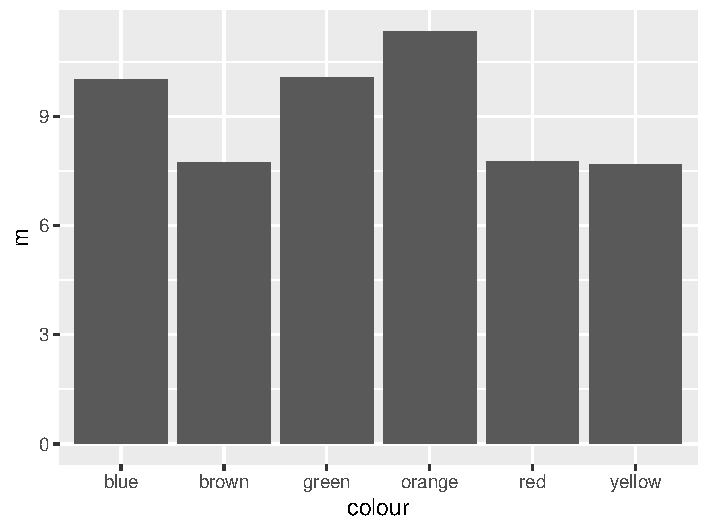
\includegraphics[scale = .75]{graphics/ch3Figs/bar_1.pdf}
\end{figure}

The argument \R{stat = "identity"} is simply telling \textit{ggplot2} to use the values within the \R{mm\_summary} data frame to create the bars.  We needed to specify this because \textit{ggplot2} has the ability to take the raw data directly (e.g., \R{mm\_data}) and perform its own summary calculations. However, we do not need it to do that in this particular case, hence why we included this argument.

You can see that what results is a bar graph representing the mean of each M\&M type. To make this look a bit nicer, we could change the fill colour of the bars to correspond to the respective colour types.\footnote{Technically, this is something we should NOT do because, for the sake of comparison, its better to give all the bars the same ``visual weight.'' Keeping all the bars the same colour does precisely that. Moreover, with the x-axis labels, there is no reason to add additional elements that could be distracting. That being said, if you are collaborating on a project, your collaborators will probably demand to see colourful bars irrespective this rationale (experience has taught me this). And if they outnumber you, they can probably beat you in a fight - it doesn't matter if you have the moral or logical high ground.} When we do this, we have to be mindful of the fact that the x-axis contains a \textit{discrete} scale, not a \textit{continuous} one like we saw in chapter 2 (for more information on discrete vs. continuous scales see section \ref{sec:pos_scale}).

First we will define our colour palette. To do this we could just specify the names of primary colours: blue, brown, green and so on. However, the actual colour of M\&M candies are slightly different than their naming scheme would suggest. The hex codes used below are much more colour accurate.

\begin{inR}
mm_palette <- c("#2f9fd7", "#603a34", "#31ac55", "#f26f22", "#b11224", "#fff200")
\end{inR}

\vspace{1em}

Once \R{my\_palette} has been created we can use it to adjust the colour of our bar graph.

\begin{inR}
ggplot(mm_summary, aes(x = type, y = m)) +
  geom_bar(
    stat = "identity",
    colour = "black",
    aes(fill = type)
  ) +
  scale_fill_discrete(type = mm_palette)
\end{inR}

\vspace{2em}

\begin{figure}[H]
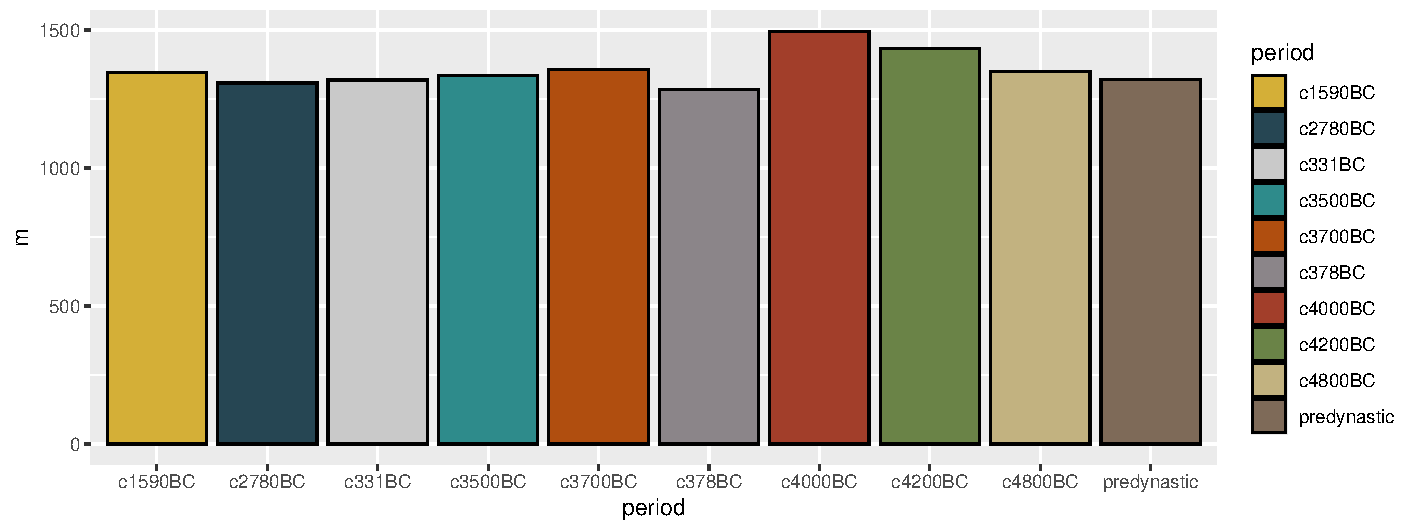
\includegraphics[scale = .75]{graphics/ch3Figs/bar_2.pdf}
\end{figure}

Now, in addition to the mean of each M\&M type, our data frame also has information pertaining to the minimum and maximum number of M\&M's (these are columns \R{\$min} and \R{\$max} respectively). We could incorporate that information in our graph with the use of \textit{errorbars}.  Errorbars are a visual representation of our data's \textit{spread}, and the difference between the minimum and maximum represent a measure of spread called the \textit{range}.\footnote{If that isn't entirely clear, don't worry. The concept of spread as a statistical term will be explained in more detail in later chapters.}

To create errorbars, we can simply use \textit{ggplot2's} \R{geom\_errorbar()} function. We just need to tell it which column corresponds to the bottom of the error bar (\R{ymin}) and which column corresponds to the top of the errorbar (\R{ymax}).

\begin{inR}
ggplot(mm_summary, aes(x = type, y = m)) +
  geom_bar(
    stat = "identity",
    colour = "black",
    aes(fill = type)
  ) +
  scale_fill_discrete(type = mm_palette) +
  geom_errorbar(aes(ymin = min, ymax = max), width = 0.25)
\end{inR}

\vspace{2em}

\begin{figure}[H]
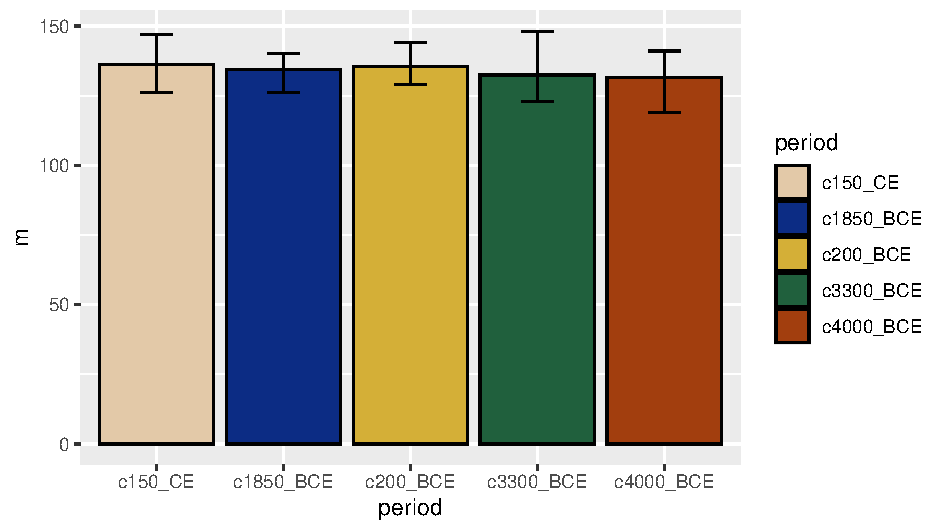
\includegraphics[scale = .75]{graphics/ch3Figs/bar_3.pdf}
\end{figure}

All that remains is to give the plot some new labelling. In other words, we should add a better x and y axis title and we should also put the x-axis labels in Title Case. The legend can be removed as well since it is redundant with the labels on the x-axis.

To change the current labels ``blue'', ``brown'', ``green'' and so on to Title Case, we can use the function \R{scale\_x\_discrete()} and use its \R{labels} argument. We just have to give it a character vector containing the new labelling (FYI: make sure you specify them in the correct order).

To remove the legend, there are different methods you could employ. In this case, since we only have the fill aesthetic mapped, it is easy enough to just add \R{guide = "none"} to the \R{scale\_fill\_discrete()} function.

\begin{inR}
ggplot(mm_summary, aes(x = type, y = m)) +
  geom_bar(
    stat = "identity",
    colour = "black",
    aes(fill = type)
  ) +
  scale_fill_discrete(type = mm_palette, guide = "none") +
  geom_errorbar(aes(ymin = min, ymax = max), width = 0.25) +
  scale_x_discrete(
    labels = c("Blue", "Brown", "Green", "Orange", "Red", "Yellow")
  ) +
  xlab("M&M Colour") +
  ylab("M&M Amount")
\end{inR}

\vspace{2em}

\begin{figure}[H]
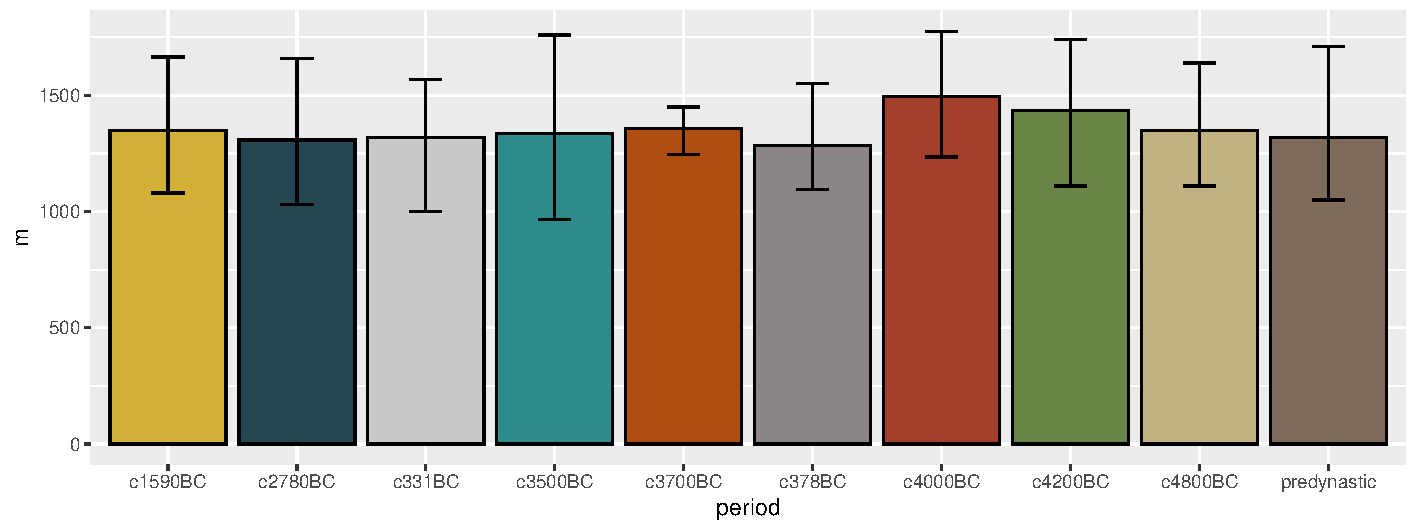
\includegraphics[scale = .75]{graphics/ch3Figs/bar_4.pdf}
\end{figure}

Having read both chapter 2 and now this current chapter, there is one key aspect of plotting that has not been dealt with yet. Specifically, how do you adjust the order of the categories? Suppose we wanted the the colours, going from left to right, to be ``red'', ``orange'', ``yellow'', ``green'', ``blue'', and ``brown''. How would we make that happen? That is where the concept of factors becomes important.

\section{Factors}

In statistics we often refer to a categorical variable as a \gls{factor},\footnote{Independent, manipulated, and predictor variables are given this label when they have a fixed set of categories or are continuous but only take on a limited number of discrete values. If this is unclear now, don't worry — variable types will be explained in more detail in a later chapter.} and factors have different \glspl{level}.  For instance, in our tidy data (\R{mm\_data}) the variable \R{\$type} could be considered a factor. Each specified colour in that column is a level of that factor: blue is its own  level, brown is its own level, green is its own level, and so on. In other words, in the M\&M data, the ``type'' factor has 6 levels.

To summarise, you can treat the term ``factor'' as synonymous with the terms ``column'' or ``variable.'' And you can treat the term ``level'' as synonymous with the term ``category.'' Though, this only applies to tidy data, not wide data.
{
\begin{itemize}
  \setlength\itemsep{-1em}
    \item Factor = column / variable
    \item Level = category within a column / variable
\end{itemize}
}

If we examine \R{mm\_data}:

\begin{inR}
mm_data
\end{inR}
\begin{outR}
# A tibble: 288 × 3
     pkg type   amount
   <dbl> <chr>   <dbl>
 1     1 blue       13
 2     1 brown       7
 3     1 green      12
 4     1 orange      9
 5     1 red         7
 6     1 yellow      8
 7     2 blue        8
 8     2 brown       3
 9     2 green      13
10     2 orange     13
# 278 more rows
\end{outR}

\noindent
You can see that the output is telling us that the \R{\$type} column is a character vector (notice the \R{<chr>}). In other words, R does not know that ``blue'', ``brown'', ``green'', etc. are categories. It just sees 278 individual character values in that particular column.

\subsection{Factoring a Column}

For the purpose of plotting and analyses, it is important that R understands ``blue'', ``brown'', ``green'', etc. are levels of a factor (i.e., it is important that it treats these as categories). We can easily tell R that a particular column is a factor using the function \R{factor()}.\footnote{Technically, when we use this function we are replacing an existing column with a new column that happens to be a factor. We are not really ``telling'' R it is a factor, we are ``creating'' a factor - but that's just a nitpicky semantic issue.}

\begin{inR}
mm_data$type <- factor(mm_data$type)

mm_data
\end{inR}
\begin{outR}
# A tibble: 288 × 3
     pkg type   amount
   <dbl> <fct>   <dbl>
 1     1 blue       13
 2     1 brown       7
 3     1 green      12
 4     1 orange      9
 5     1 red         7
 6     1 yellow      8
 7     2 blue        8
 8     2 brown       3
 9     2 green      13
10     2 orange     13
# 278 more rows
\end{outR}


\noindent
Notice that now the column \R{\$type} is now listed as \R{<fct>}, which stands for ``factor.''  Moreover, if we isolate the column after doing this ...

\begin{inR}
mm_data$type
\end{inR}
\begin{outR}
...
[261] green  orange red    yellow blue   brown  green  orange red    yellow
[271] blue   brown  green  orange red    yellow blue   brown  green  orange
[281] red    yellow blue   brown  green  orange red    yellow
Levels: blue brown green orange red yellow
\end{outR}

\noindent
You can see at the bottom of the output, that the six levels of our factor have been specified. Generally speaking, to view the levels of a factor, a better practice is to use the \R{levels()} function.

\begin{inR}
levels(mm_data$type)
\end{inR}
\begin{outR}
[1] "blue"   "brown"  "green"  "orange" "red"    "yellow"
\end{outR}

\subsection{Ordering Levels}

Discerning readers will have noticed that the order of the levels here (from left to right) matches the order of the bars on the plot we made earlier. This is because anytime you plot or summarise categories using \textit{ggplot2} and \textit{dplyr} functions respectively, these packages silently factor the data behind the scenes and R's default behaviour is to put factors in alphabetical order (which is why we saw the order we did).  But we can change the order by specifying it inside the factor function.

\begin{inR}
mm_data$type <- factor(mm_data$type,
  levels = c("red", "orange", "yellow", "green", "blue", "brown")
)

levels(mm_data$type)
\end{inR}

\begin{outR}
[1] "red"    "orange" "yellow" "green"  "blue"   "brown" 
\end{outR}

It is important to emphasize that this does not change anything about how the data is laid out in our data frame. All those values are still in the same order. All we are doing here is telling R that, when it does it any analyses or plotting, that ``red'' comes before ``orange'' which comes before ``yellow'', and so on. For instance, when we re-run our earlier code that created the summary statistic data, you can see that the \R{\$type} column now follows this new order we have specified.

\begin{inR}
mm_summary <- mm_data |>
  group_by(type) |>
  summarise(
    m = mean(amount),
    tot_type = sum(amount),
    tot_overall = sum(mm_data$amount),
    percent = tot_type / tot_overall * 100,
    min = min(amount),
    max = max(amount)
  )

mm_summary
\end{inR}

\begin{outR}
# A tibble: 6 × 7
  type       m tot_type tot_overall percent   min   max
  <fct>  <dbl>    <dbl>       <dbl>   <dbl> <dbl> <dbl>
1 red     7.75      372        2620    14.2     2    12
2 orange 11.3       544        2620    20.8     7    17
3 yellow  7.69      369        2620    14.1     2    14
4 green  10.1       483        2620    18.4     5    17
5 blue   10.0       481        2620    18.4     5    16
6 brown   7.73      371        2620    14.2     3    12
\end{outR}

\noindent

Moreover, when we now plot the data the bars will also have shifted their position accordingly.

\begin{inR}
ggplot(mm_summary, aes(x = type, y = m)) +
  geom_bar(stat = "identity")
\end{inR}

\vspace{2em}

\begin{figure}[H]
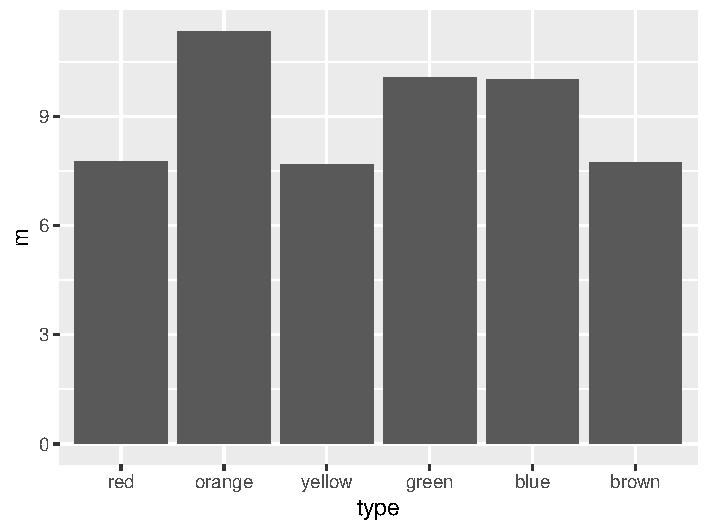
\includegraphics[scale = .75]{graphics/ch3Figs/bar_5.pdf}
\end{figure}

\subsection{Naming Levels}

On occasion, it will be useful to rename the levels of a factor. For instance, all of our levels are currently lower case, but to make them title case we could use the \R{levels()} function from earlier.

\begin{inR}
levels(mm_summary$type) <- c("Red", "Orange", "Yellow", "Green", "Blue", "Brown")

mm_summary
\end{inR}
\begin{outR}
# A tibble: 6 × 7
  type       m tot_type tot_overall percent   min   max
  <fct>  <dbl>    <dbl>       <dbl>   <dbl> <dbl> <dbl>
1 Red     7.75      372        2620    14.2     2    12
2 Orange 11.3       544        2620    20.8     7    17
3 Yellow  7.69      369        2620    14.1     2    14
4 Green  10.1       483        2620    18.4     5    17
5 Blue   10.0       481        2620    18.4     5    16
6 Brown   7.73      371        2620    14.2     3    12
\end{outR}

\noindent
A corresponding change will be seen on the plot's x-axis labels as well when that is generated.

A word of warning is needed here. DO NOT confuse the \R{levels} \textit{argument} inside \R{factor()} function with the \R{levels()} \textit{function}. The \R{levels} argument is used for ordering levels. The \R{levels()} function is for re-naming levels.\footnote{At the risk of confusing readers, I feel obligated to mention that the \R{factor()} function has an additional argument \R{labels} that will allow you to change the level names. See R documentation: \R{?factor}}

{
\begin{itemize}
    \item Ordering levels: \R{factor(df\$column, levels = c(new order))}
    \item Naming levels: \R{levels(df\$column) <- c(new names)}
\end{itemize}
}

Particularly for beginners, factors are annoying to contend with, but they are vital for so many things within R and therefore a necessary evil. Consequently, it is recommended to new users that they submit and wholeheartedly embrace this wickedness. Only then will they find inner peace with factoring.
